\item O bloco de \SI{50}{\kilogram} é transportado por uma distância curta, usando-se dois rolos cilíndricos, cada um
com massa de \SI{17.5}{\kilogram}. Se uma força horizontal $P=\SI{125}{\newton}$ é aplicada ao bloco, determine a velocidade
dele após haver se deslocado \SI{.6}{\meter} para a esquerda. Originalmente o bloco está em repouso. Não há deslizamento.

\begin{flushright}
	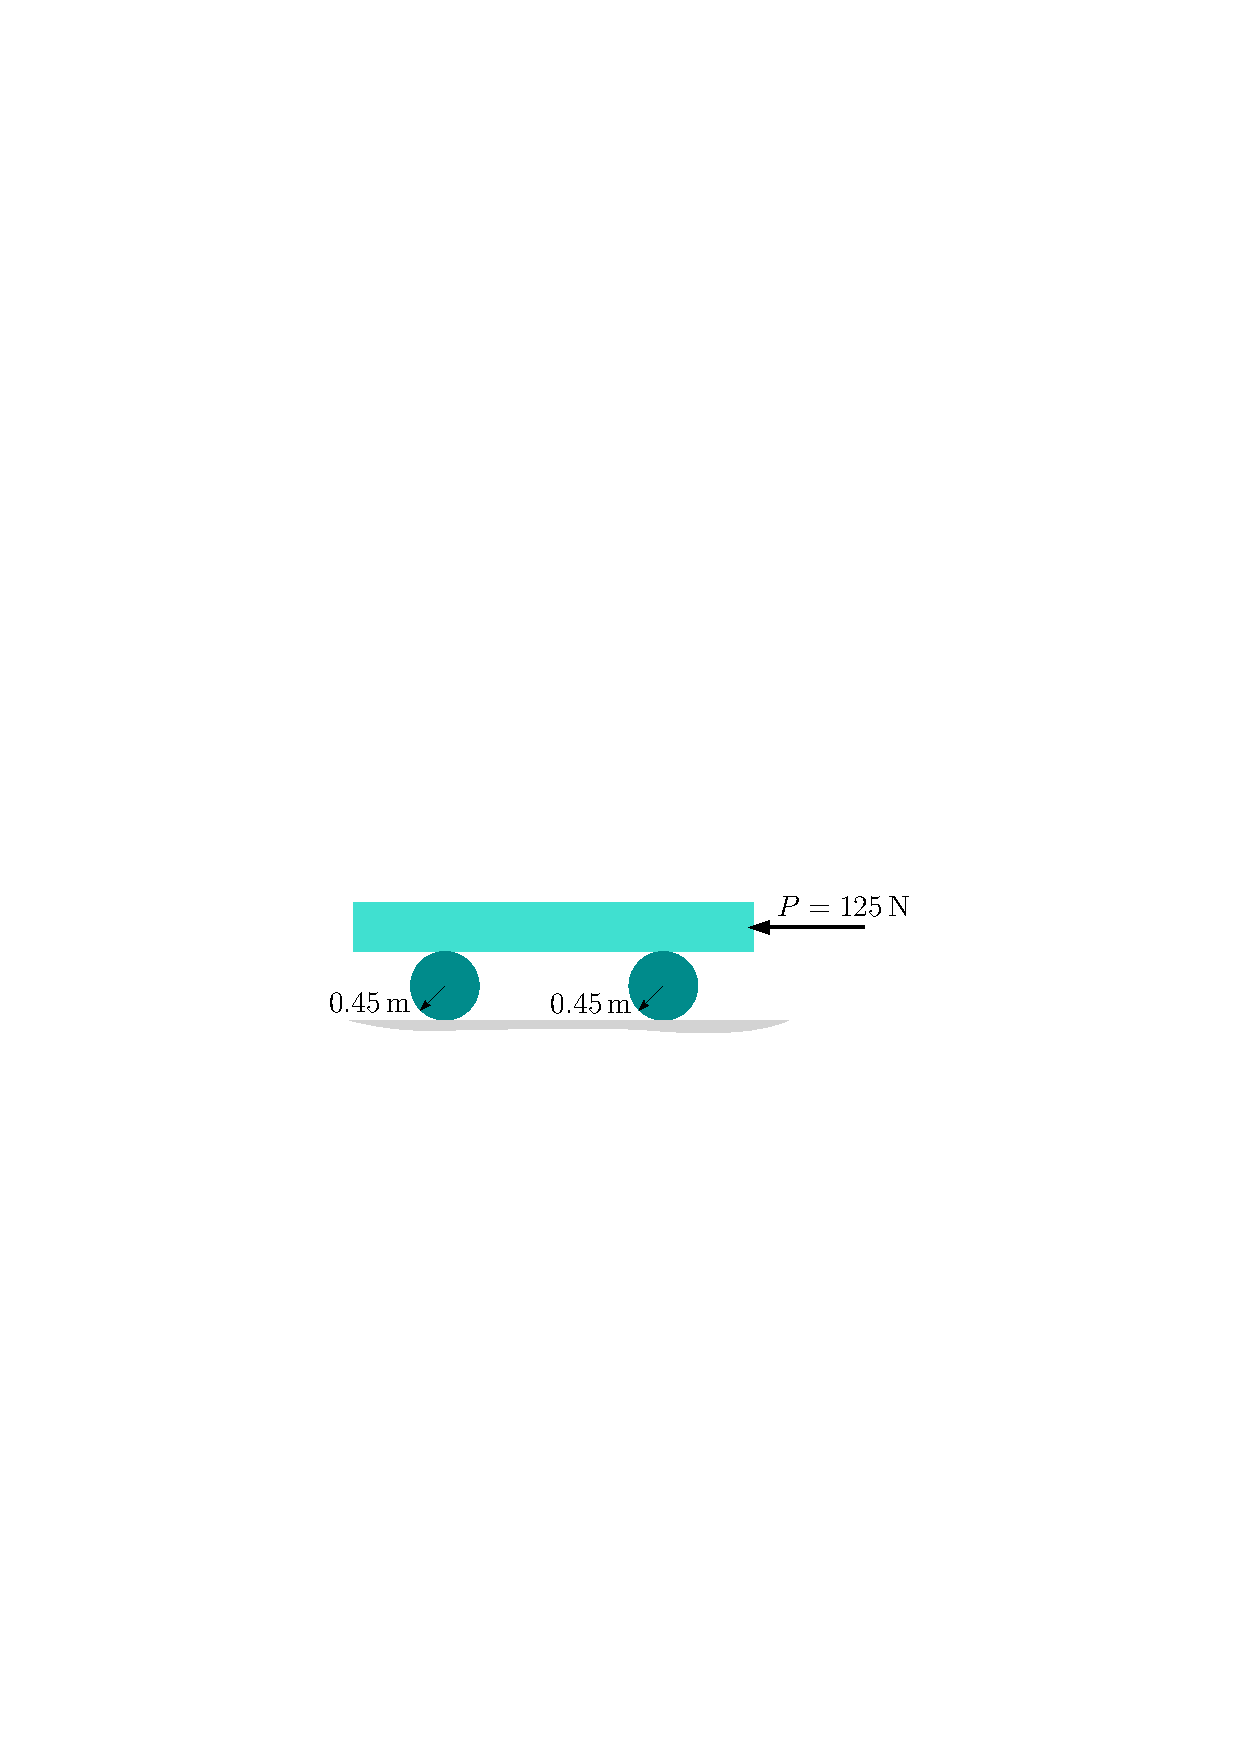
\includegraphics[scale=.8]{../../images/draw_4}
\end{flushright}